% !TEX TS-program = lualatex
\documentclass{standalone}
\usepackage{tikz, pgfplots, amssymb, amsmath, amsfonts}
\pgfplotsset{compat=1.18}
\newcommand{\vect}[1]{\boldsymbol{\mathbf{#1}}}
\begin{document}
\begin{tikzpicture}
    \begin{axis}[
        ymin=0,ymax=1,
        xmin=0, xmax=1,
        xlabel={Complessità},
        ylabel={Errore},
    ]
    \draw
        (0.05,0.7)node[circle, draw, purple, fill=purple, inner sep=1.5pt]{}
        (0.1,0.6)node[circle, draw, blue, fill=blue, inner sep=1.5pt]{}
        (0.2,0.5)node[circle, draw, black, fill=black, inner sep=1.5pt]{}
        (0.5,0.25)node[circle, draw, black, fill=black, inner sep=1.5pt]{}
        (0.7,0.2)node[circle, draw, fill=green, green, inner sep=1.5pt]{}
        
    ;
        
    \end{axis}
\end{tikzpicture}
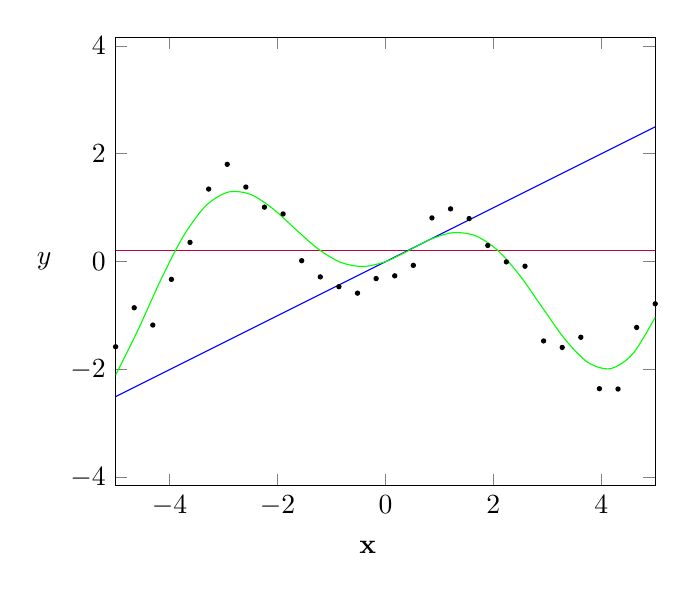
\begin{tikzpicture}
    \begin{axis}[
        view={0}{90},
        axis equal, 
        xmin=-5, xmax=5,
        ymin=-2.5,ymax=2.5,
        xlabel={$\vect{x}$\textcolor{white}{Cp}},
        ylabel={$y$},
        ylabel style={rotate=-90}
    ]
    \addplot[only marks, samples=30, mark size=0.75]{0.5*x*sin(-180*(x+4)/pi)+0.6*rand};
    \addplot[blue, smooth, domain=-5:5, purple]{0.2} node[pos=0.95](f1){};
    \addplot[blue, smooth, domain=-5:5, blue]{0.5*x} node[pos=0.95](f2){};
    \addplot[blue, smooth, domain=-5:5, green]{0.5*x*sin(-180*(x+4)/pi)} node[pos=0.95](f2){};
    \end{axis}
\end{tikzpicture}
\end{document}